% ---------------------------------------------------------------------------
% Author guideline and sample document for EG publication using LaTeX2e input
% D.Fellner, v1.22, Jan 22, 2024

\documentclass{egpubl}
 
% --- for  Annual CONFERENCE
% \ConferenceSubmission   % uncomment for Conference submission
% \ConferencePaper        % uncomment for (final) Conference Paper
% \STAR                   % uncomment for STAR contribution
% \Tutorial               % uncomment for Tutorial contribution
% \ShortPresentation      % uncomment for (final) Short Conference Presentation
% \Areas                  % uncomment for Areas contribution
% \Education              % uncomment for Education contribution
\Poster                 % uncomment for Poster contribution
% \DC                     % uncomment for Doctoral Consortium
%
% --- for  CGF Journal
% \JournalSubmission    % uncomment for submission to Computer Graphics Forum
% \JournalPaper         % uncomment for final version of Journal Paper
%
% --- for  CGF Journal: special issue
% \SpecialIssueSubmission    % uncomment for submission to , special issue
% \SpecialIssuePaper         % uncomment for final version of Computer Graphics Forum, special issue
%                          % EuroVis, SGP, Rendering, PG
% --- for  EG Workshop Proceedings
% \WsSubmission      % uncomment for submission to EG Workshop
% \WsPaper           % uncomment for final version of EG Workshop contribution
% \WsSubmissionJoint % for joint events, for example ICAT-EGVE
% \WsPaperJoint      % for joint events, for example ICAT-EGVE
% \WsPaperJointdemo         % uncomment for final version of EG Workshop contribution
% \WsPaperJointposter         % uncomment for final version of EG Workshop contribution 
% \WsPoster          % uncomment for Poster contribution
% \WsShortPaper      % uncomment for Short Paper contribution
% \Expressive        % for SBIM, CAe, NPAR
% \DigitalHeritagePaper
% \PaperL2P          % for events EG only asks for License to Publish

% --- for EuroVis 
% for full papers use \SpecialIssuePaper
% \STAREurovis   % for EuroVis additional material 
% \EuroVisPoster % for EuroVis additional material 
% \EuroVisShort  % for EuroVis additional material
% \MedicalPrize  % uncomment for Medical Prize (Dirk Bartz) contribution, since 2021 part of EuroVis
% \EuroVisEducation              % uncomment for Education contribution

% Licences: for CGF Journal (EG conf. full papers and STARs, EuroVis conf. full papers and STARs, SR, SGP, PG)
% please choose the correct license
% \CGFStandardLicense
%\CGFccby
%\CGFccbync
%\CGFccbyncnd

% !! *please* don't change anything above
% !! unless you REALLY know what you are doing
% ------------------------------------------------------------------------
\usepackage[T1]{fontenc}
\usepackage{graphicx}
\usepackage{dfadobe}  
\usepackage{tikz}
\usepackage{overpic}
\usepackage{amsmath}
\usepackage{amssymb}
\usepackage{float}
\usepackage{cite}  % comment out for biblatex with backend=biber
\usetikzlibrary{arrows, decorations.markings, arrows.meta,positioning,shadows,shapes.geometric,automata,positioning,fit,arrows.meta,calc,bending}



% ---------------------------
%\biberVersion
\BibtexOrBiblatex
%\usepackage[backend=biber,bibstyle=EG,citestyle=alphabetic,backref=true]{biblatex} 
%\addbibresource{egbibsample.bib}

%%%the style file EG-sub.bbx does not truncate authors' list to 3 if number of authors are more than 4.
%%%This is important for checking conflicts during review assigment phase. For final version please use EG.bbx,
%%%using et al. for more then 4 authors.

% ---------------------------  
\electronicVersion
\PrintedOrElectronic
% for including postscript figures
% mind: package option 'draft' will replace PS figure by a filename within a frame

\usepackage{egweblnk} 
% end of prologue

% ---------------------------------------------------------------------
% EG author guidelines plus sample file for EG publication using LaTeX2e input
% D.Fellner, v2.04, Dec 14, 2023


\title[EG poster]%
      {Markerless Multi-person Pose Estimation and Motion Synthesis for Combat Sports}

% for anonymous conference submission please enter your SUBMISSION ID
% instead of the author's name (and leave the affiliation blank) !!
% for final version: please provide your *own* ORCID in the brackets following \orcid; see https://orcid.org/ for more details.
\author[Hossein]
{\parbox{\textwidth}{\centering 
        Hossein Feiz$^1$, David Labbé$^2$, Sheldon Andrews$^3$
        }
        \\
{\parbox{\textwidth}{\centering 
        École de technologie supérieure (ETS), Montreal, Canada
       }
}
}
% ------------------------------------------------------------------------

% if the Editors-in-Chief have given you the data, you may uncomment
% the following five lines and insert it here
%
% \volume{36}   % the volume in which the issue will be published;
% \issue{1}     % the issue number of the publication
% \pStartPage{1}      % set starting page


%-------------------------------------------------------------------------
\begin{document}

% uncomment for using teaser
\teaser{
 \includegraphics[width=0.9\linewidth]{pipeline.pdf}
 \centering
  \caption{The pipeline begins with generating bounding boxes  and robust tracking  for each individual in the scene. These tracking results are used to produce 2D poses using ViTPose. The triangulation process, produces smooth 3D keypoints. The kinematics optimization step incorporates the 2D and 3D keypoints, to create the SMPL parameters ($\mathbf{\theta}$, $\mathbf{\beta}$). The 3D relative joint positions , initial pose state  and velocity state of the humanoid , serve as a reference for a dynamic optimizer to correct any artifacts in the motion.}
\label{fig:teaser}
}

\maketitle
%-------------------------------------------------------------------------

\begin{abstract}
   Combat sports pose significant challenges for motion capture due to dynamic interactions and crowded backgrounds. Traditional methods like optical marker tracking, IMU-based solutions are not practical due to their intrusive nature, and Monocular vision-based approaches are hindered by occlusions, prompting the development of a multi-stage, multi-view tracking pipeline. This pipeline utilizes kinematic optimization to fuse 2D keypoints from multiple cameras, followed by physics-based trajectory optimization using model predictive control to enhance realism.
   Furthermore, leveraging interaction datasets attain from multi-view setup, the pipeline supports multi-person motion synthesis. It employs a seq2seq model to generate interactions from sparse VR headset inputs, and the whole body poses. Finally, latent optimization ensures motions adhere to motion prior and satisfies high level criteria to lifelike animations suitable for combat sports analysis and training applications.

\begin{CCSXML}
<ccs2012>
<concept>
<concept_id>10010147.10010371.10010352.10010381</concept_id>
<concept_desc>Computing methodologies~Pose Estimation</concept_desc>
<concept_significance>300</concept_significance>
</concept>
<concept>
<concept_id>10010147.10010371.10010352.10010382</concept_id>
<concept_desc>Computing methodologies~Motion synthesis</concept_desc>
<concept_significance>300</concept_significance>
</concept>
</ccs2012>
\end{CCSXML}

\ccsdesc[300]{Computing methodologies~Pose Estimation}
\ccsdesc[300]{Computing methodologies~Motion synthesis}


\printccsdesc   
\end{abstract}  
%-------------------------------------------------------------------------
\section{Introduction}


\section{Pose Estimation}

\textbf{Tracking 2D and 3D Data:} Using epipolar constraints and long-term video object segmentation Triangulation computes 3D positions from 2D keypoints across multiple cameras using their projection matrices. It solves a linear system to determine 3D coordinates, weighting contributions based on 2D keypoints’ confidence. Techniques like SVD solve this system, with subsequent filtering and smoothing ensuring robust 3D reconstructions, even in the presence of noise and outliers.

\textbf{Kinematics Optimization:} The kinematics optimization methodology discussed focuses on refining the pose estimation of athletes using a hybrid approach of 2D and 3D keypoint data. Employing the SMPL model, the optimization aims to minimize the disparity between model joints and observed data while ensuring temporal coherence and natural movement. This is achieved through a comprehensive objective function that includes terms for smoothness, similarity to human motion priors, and alignment with both 2D re-projection evidence and triangulated 3D keypoints.

Initially, the optimization initializes shape parameters ($\beta \in \mathbb{R}^{10}$) of the SMPL model based on 3D keypoints obtained through triangulation. Subsequently, it iteratively adjusts these parameters alongside pose parameters ($\theta \in \mathbb{R}^{72}$) to refine the pose estimation. The process integrates a Limited-memory Broyden–Fletcher–Goldfarb–Shanno (LBFGS) optimizer, configured with specific parameters for efficient minimization of the objective function.

Key components of the objective function include:

\begin{itemize}
    \item \textbf{2D Re-projection Loss} ($\mathrm{L}_\text{2D}$): Aligns 3D joints with 2D joints across multiple camera views, emphasizing joints with high-confidence detections using a robust error function.
    \item \textbf{3D Alignment Loss} ($\mathrm{L}_\text{3D}$): Computes the Euclidean distance between predicted 3D joint positions and triangulated 3D keypoints, weighted by their confidence scores.
    \item \textbf{Smoothness Loss} ($\mathrm{L}_\text{smooth}$): Promotes consistency in pose transitions over time frames and vertices of the posed mesh.
    \item \textbf{Prior Losses} ($\mathrm{L}_{\text{GMM}}$, $\mathrm{L}_{\text{Vposer}}$): Introduces Gaussian Mixture Model (GMM) and Vposer priors to penalize unnatural poses, guiding the optimization towards more realistic and fluid motion.
\end{itemize}

Through experimental validation, the inclusion of these priors has proven effective in reducing limb jitter and enhancing the overall naturalness of the optimized poses. This comprehensive approach ensures accurate and lifelike pose estimation suitable for applications in sports biomechanics and animation.

\begin{figure}[htbp]
  \centering

  \begin{figure}[H]
  \centering
  \resizebox{\columnwidth}{!}{%
 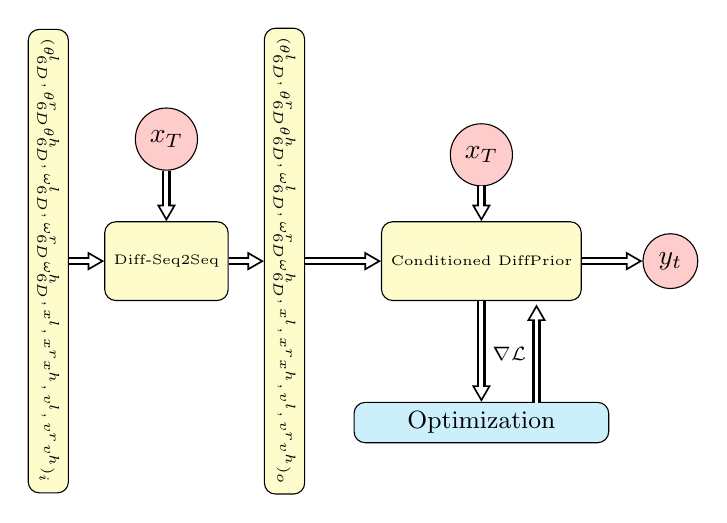
\begin{tikzpicture}[node distance=2cm]
\tikzstyle{process}=[draw, font=\fontsize{5}{4.8}\selectfont, rectangle, rounded corners, fill=yellow!20, minimum width=1cm, auto, on grid, minimum height=1cm, align=center]
\tikzstyle{process4}=[draw, font=\small, rectangle, rounded corners, fill=yellow!20, text width=3cm, auto, on grid, align=center]
\tikzstyle{decision}=[draw, font=\small, rectangle, rounded corners, fill=red!20, text width=3cm, auto, on grid, align=center]
\tikzstyle{process2}=[draw, font=\small, rectangle, rounded corners, fill=cyan!20, text width=3cm, auto, on grid, align=center]
\tikzstyle{circlenode}=[draw, circle, fill=red!20, minimum size=1mm]
\tikzstyle{process3}=[draw, font=\fontsize{5}{4.8}\selectfont, rectangle, rounded corners, fill=cyan!20, rotate=-90, auto, on grid, align=center]
\tikzstyle{process4}=[draw, font=\fontsize{5}{4.8}\selectfont, rectangle, rounded corners, fill=yellow!20, rotate=-90, auto, on grid, align=center]
\tikzstyle{vecArrow} = [thick, decoration={markings, mark=at position 1 with {\arrow[semithick]{open triangle 60}}}, double distance=1.4pt, shorten >= 5.5pt, preaction = {decorate}, postaction = {draw, line width=1.4pt, white, shorten >= 4.5pt}]
\tikzstyle{vecArrow1} = [thick, decoration={markings, mark=at position 0.9 with {}}, double distance=1.4pt, shorten >= 5.5pt, preaction = {decorate}, postaction = {draw, line width=1.4pt, white, shorten >= 4.5pt}]
\tikzstyle{innerWhite} = [semithick, white, line width=1.4pt, shorten >= 4.5pt]

\node[process4] (input) at (-4.5, -0.35) {$(\theta_{6D}^{l}, \theta_{6D}^{r} \theta_{6D}^{h}, \omega_{6D}^{l}, \omega_{6D}^{r} \omega_{6D}^{h}, x^{l}, x^{r} x^{h}, v^{l}, v^{r} v^{h})_i$};
\node[process] (seq2seq) at (-3, -0.35) {Diff-Seq2Seq};
\draw[vecArrow] (input) -- (seq2seq);
\node[process4] (output) at (-1.5, -0.35) {$(\theta_{6D}^{l}, \theta_{6D}^{r} \theta_{6D}^{h}, \omega_{6D}^{l}, \omega_{6D}^{r} \omega_{6D}^{h}, x^{l}, x^{r} x^{h}, v^{l}, v^{r} v^{h})_o$};
\draw[vecArrow] (seq2seq) -- (output);
\node[process] (prior) at (1, -0.35) {Conditioned DiffPrior};
\node[circlenode] (yt) at (3.4, -0.35){$y_t$};
\node[circlenode] (xt) at (1, 1){$x_T$};
\node[circlenode] (xt1) at (-3, 1.2){$x_T$};
\draw[vecArrow] (prior) -- (yt);
\draw[vecArrow] (xt1) -- (seq2seq);
\draw[vecArrow] (xt) -- (prior);

\draw[vecArrow] (output) -- (prior);
\node[process2] (optimization) at (1, -2.4) {Optimization};
\draw[vecArrow] (prior) -- (optimization);
\draw[vecArrow] (1.7, -2.15) tonode[anchor=east] {\scriptsize $\nabla \mathcal{L}$} (1.7, -0.9);

\end{tikzpicture}
  }
\end{figure}

  \caption{\label{fig:condtion-diffusion}
           The condition for the seq2seq model contains the VR sensor information of the player and the output is the corresponding VR sensor input for the opponent at each sequence. The conditional diffusion prior is conditioned on the opponent synthetic information and produces the whole body pose for the opponent. The optimization in loop make sure the output motion has the desired trajectories based on a loss function.}
\end{figure}

Figure~\ref{fig:condtion-diffusion} which need the full textwidth can be typeset as Figure.

%-------------------------------------------------------------------------
\textbf{Dynamics Optimization:} In the described study, a two-stage optimization approach is employed to enhance the accuracy and quality of motion tracking for athletes. The initial stage focuses on kinematic optimization, which estimates full-body poses but often introduces high-frequency artifacts known as jitter. To mitigate this, a second stage employs dynamics optimization using a physics-based humanoid model. This model, derived from joint positions and landmarks of an SMPL mesh, creates an articulated rigid-body structure with capsule collision geometry, featuring 56 joint-angle degrees of freedom and a 6 degree of freedom root joint.

The dynamics optimization stage aims to refine motion trajectories by considering joint torques and biomechanical constraints within a physical environment. It computes joint torques using an iterative Linear Quadratic Regulator (iLQR) algorithm, which optimizes control inputs to smooth and stabilize motion trajectories while adhering to physical realism. This approach accounts for contact forces and body dynamics, enhancing the overall quality and naturalness of the generated motions.

Furthermore, trajectory optimization in this framework minimizes a weighted sum of regularization terms and loss functions, which include penalties for velocity and control values. By iteratively refining control trajectories over short time horizons, the method achieves improved alignment with desired motion characteristics derived from the kinematic stage outputs. Overall, this integrated approach ensures robust and realistic motion tracking suitable for applications in sports biomechanics and animation.

\section{Motion Synthesis}
%---------------------------------------------------------------------
\textbf{Interaction Diffusion Model:}
 
A novel application of sequence-to-sequence (seq2seq) models in virtual reality involves generating responsive opponent motions based on sparse VR input data. In this context, the seq2seq model serves as a pivotal tool for translating sparse signals captured from VR sensors into realistic and dynamic movements for virtual opponents. Trained on a specialized multi-person boxing dataset, the model learns to map the sparse input, which could include data from wearable IMUs or HMDs, into coherent sequences of actions that simulate human-like behavior during a boxing match. By leveraging the dataset’s diverse scenarios and real-world motion variations, the seq2seq model not only predicts the opponent’s reactions but also adapts to different player actions, enhancing the realism and engagement of VR gaming experiences. This approach marks a significant advancement in interactive VR applications by bridging the gap between sparse sensor data and immersive virtual interactions, thereby enriching the user experience through responsive and lifelike virtual opponents.
%---------------------------------------------------------------------
\textbf{Conditioned Diffprior:}
The application of conditional diffusion models, specifically tailored for full-body motion synthesis from sparse IMU tracking signals, represents a breakthrough in virtual reality (VR) body tracking. This approach overcomes the inherent challenges of accurately predicting smooth and realistic full-body motions with minimal input data. By leveraging a lightweight MLP architecture and employing a block-wise injection scheme for embedding time step information, the conditional diffusion model effectively reduces artifacts like jittering and enhances robustness against signal loss. These advancements are underscored by its superior performance on benchmarks like the AMASS dataset, setting new standards in motion prediction methods.

In parallel, the conditional diffusion model paradigm also finds application in frameworks designed for real-time human motion tracking in VR environments. This innovative approach integrates scalable 3DOF IMUs with head-mounted displays (HMDs), offering a flexible solution that balances tracking accuracy with user-friendliness across various VR setups. Central to its efficacy is a lightweight temporal-spatial feature learning (TSFL) network, combining LSTM for temporal feature capture and Transformer for spatial correlation learning. This hybrid architecture optimizes computational efficiency while maintaining high accuracy in estimating full-body poses, making it suitable for immersive VR experiences demanding fluid and responsive interactions.

%---------------------------------------------------------------------
\textbf{Latent Optimization:}

Optimize noisy motion inputs directly in the latent space of the diffusion model. By treating motion denoising as a black box and iteratively adjusts the diffusion noise vector using gradients computed through an ODE solver, ensuring the output motion meets user-defined criteria. This approach avoids the need for fine-tuning models for specific tasks, demonstrating superior performance in motion editing, preservation, and task fulfillment compared to existing methods.

\end{document}
{}
